\chapter{Clustering}\label{chap:clustering}

In this part of the thesis, we used clustering methods to improve the performance of the previous prediction models. The goal is to find groups of data points that are similar to each other but different from the rest of the data. This is done by finding the distance between each data point and the rest of the data. Most algorithms calculate the distance between two data points using a distance metric.

In this chapter, the clustering methods that were used will be briefly explained in section \ref{sec:clustering_methods}. Section \ref{sec:validity_measures} provides an overview of the clustering validity metrics used in this work. Section \ref{sec:clustering_experiments} presents the experiments undertaken to determine the most appropriate clustering method for the dataset. Section \ref{sec:clustering_ml_experiments} explains the experiments undertaken with the solar wind prediction model with the most appropriate clustering from the previous task. Finally, Section \ref{sec:clustering_summary} provides an overview of the work in this chapter.
%

\section{Clustering Methods}\label{sec:clustering_methods}
Clustering is defined as finding and then grouping the data values that are close to each other in some way. Due to these reasons, clustering works as a valuable technique not only for data analysis but also for enhancing machine learning performance. Additionally, clustering can be used for anomaly detection, as abnormal samples tend to be far from the rest of the data. In this section, the clustering methods that were used in this work will be presented.

There are several approaches to the clustering task; however, these can be divided into two main categories: Hierarchical and Partitional. In the hierarchical approach, the data is iteratively divided in accordance with its patterns in a bottom or top-down approach. This category is further subdivided into agglomerative and divisive techniques. For the first, clusters start at a single point and are iteratively merged with other points forming increasingly larger clusters. On the other hand, the divisive approach starts with all the data points in a single cluster and then divides them into smaller clusters. These methods tend to originate dendrograms representing the nested grouping of patterns and similarity levels. \cite{Jain.Murty.ea_Dataclusteringreview_1999a, Saxena.Prasad.ea_reviewclusteringtechniques_2017}

The Partitional approach divides the data into a set of non-overlapping clusters. These methods are usually based on optimising a criterion function, such as minimising the sum of squared errors. The most common methods in this category are K-Means and K-Medoids. This category can also be subdivided into distance, density and model-based approaches. The distance approach divides the data into clusters based on the distance between the data points, such as in the KMeans method. Density-based approaches are based on the idea that clusters are dense regions of data points that are separated by regions of lower density. Model-based approaches often apply decision trees or neural networks to learn the patterns in the data and then use these models to cluster the data. \cite{Saxena.Prasad.ea_reviewclusteringtechniques_2017}


\subsection{K-Means}\label{sec:kmeans} 
K-Means aims to find a partition of the data into K clusters, where each data point belongs to the cluster with the nearest mean. The K-means algorithm is an iterative algorithm randomly assigning each data point to a cluster. Then, the mean of each cluster is calculated, and the data points are reassigned to the cluster with the nearest mean. This process is repeated until the data points stop changing clusters. 

The number of divisions is defined by the $k$ parameter, which can be determined with the help of the Elbow Test, a heuristic method used to find the optimal number of clusters. This method plots the sum of squared errors (SSE) for each value of $k$ and then finds the value of $k$ that has the "elbow" in the plot. This value of $k$ is considered to be the optimal number of clusters. This method presents some disadvantages, as it is not always clear where the "elbow" is, making it a subjective method. Also, the SSE is not a good measure of the clustering quality, as it is biased towards clusters of similar sizes.

K-means is advantageous compared to other clustering methods because of its simplicity and the fact that it doesn't require any prior knowledge of the data. However, the disadvantages are that it is biased towards spherical clusters with similar sizes, is sensitive to the initial position of cluster centroids and requires the determination of the number of clusters beforehand.

\subsection{SOM}\label{sec:som}
This method is based on the idea of self-organizing maps, which are artificial neural networks used to find a low-dimensional representation of a high-dimensional space. It is usually employed to reduce the dimensions of the data to a map but can also be used as a clustering method, as it groups similar data. 

Unlike other neural network algorithms, SOM is trained with competitive learning. In this method, neurons compete to be the most similar to the data point. This point can only cause the activation of a single neuron in the network, called the \textit{Best Matching Unit} (BMU). At the end of the training process, each neuron is specialized in a specific region of the input space, presenting a cluster.

The algorithm starts by randomly assigning each data point to a neuron in the map. Next, a random input vector is chosen from the dataset, and the BMU is determined. This is done by measuring the distance between each neuron's input vector and weight vectors and then choosing the neuron with the minimum distance to the input. The BMU and its neighbours are then updated to be more similar to the input vector. This process is repeated until the map converges. 


The advantage of this algorithm is that it can map high-dimensional input vectors to a low-dimensional space while preserving the original topology of the data. Unlike other clustering methods, which cannot provide good results for data with high dimensionality.\footnote{Self-Organizing Maps \url{https://sites.pitt.edu/~is2470pb/Spring05/FinalProjects/Group1a/tutorial/som.html}}

\subsection{Agglomerative Clustering}\label{sec:aglomerative}
Agglomerative clustering is a hierarchical clustering method that assigns each data point to its cluster. Then, the two closest to each other are merged into a single cluster. This process is repeated until all the data points are in the same cluster. These are combined by comparing intra-cluster and inter-cluster distances. Distance between the clusters is calculated using a linkage function, and the distance between the data points in the clusters is calculated using a distance metric (normally the Euclidean distance). These two parameters directly influence the size and shape of the clusters.

The number of clusters can be determined with the help of a dendrogram plot. This plot shows the distance between the clusters as they are merged. Each leaf in the dendrogram represents a data point fused with a similar point into the same cluster as the height of the tree increases. The height of the fusion (on the vertical axis) represents the dissimilarity score between the two clusters. Higher fusions indicate that the clusters are more distinct. As a rule of thumb, the number of clusters can be determined by looking at the height of the fusion(s) with the most distinct clusters (higher dissimilarity scores).\footnote{Agglomerative Clustering \url{https://www.datanovia.com/en/lessons/agglomerative-hierarchical-clustering/}}

One of the problems with this method is that there is no clear way to determine the number of clusters, as the dendrogram doesn't always produce clear divisions, making choosing the number of clusters subjective.

\subsection{DBSCAN}\label{sec:dbscan}
This unsupervised clustering method was first introduced in Ester et al. \cite{dbscan}. It is a density-based clustering algorithm used to find clusters of data points close to each other. The algorithm assigns "core" labels to the points with at least $minPts$ points within a distance $eps$ from them. Points that are reachable from a core point, but do not have at least $minPts$ points within a distance $eps$ from them, are assigned "border" labels. These are considered part of the cluster formed by the core point. Points not reachable from any core point are assigned "noise" labels and are considered outliers. Because of this, the algorithm provides a basic method for outlier detection.

The algorithm is advantageous because it doesn't require determining the number of clusters beforehand, as it can find clusters of any size and is also robust to outliers. Despite this, it is sensitive to the parameters $minPts$ and $eps$, with slight changes in these parameters significantly impacting the results.

\section{Validity Measures\label{sec:validity_measures}}
As previously stated, one of the main difficulties in clustering is deciding the right number of clusters to ensure a clear data division. This is a subjective process in which the use of validity measures can aid. These measures, often called indices, are used to evaluate the quality of the clustering and can be used to determine the optimal number of clusters. In this section, the validity measures that were used in this work will be presented.

Cluster validity indices can be divided into three categories: external, internal and relative. External validity indices compare the clustering results with the ground truth (labels). On the other hand, internal validity indices serve to evaluate the quality of the clustering without the use of external information. Relative validity evaluates the clustering structure by varying different parameters of the algorithm, such as the number of clusters.

External validity criteria will not be considered for this study as no ground truth information is available. Instead, internal and relative validity approaches will be used to evaluate the clustering quality. The internal validity indices that were used are the following:
\\

\noindent\textbf{Silhouette Score (S).} This score is among the most widely used to evaluate clustering goodness. It is also called the mean Silhouette Coefficient for all clusters and is calculated with the mean intra-cluster distance and the mean nearest-cluster distance. Observations with a score close to 1 are well clustered, while observations close to -1 are likely to be assigned to the wrong cluster. Scores around 0 indicate overlapping clusters.
\\

\noindent\textbf{Calinski-Harabasz Index (CH).} This index is also known as the Variance Ratio Criterion. It is calculated by dividing the between-cluster or inter-cluster dispersion by the within-cluster or intra-cluster dispersion. The higher the value of the index, the better the clustering. Like the silhouette score, it evaluates the goodness of the clustering structure, with higher values indicating better clustering; contrary to the previous score, it has no reasonable bound and can take any value. Because of this, it is difficult to use this metric to compare clusterings generated with different methods.
\\

\noindent\textbf{Davies-Bouldin Index (DB).} This index is calculated by taking the average similarity measure of each cluster with its most similar cluster. This is done by calculating intra-cluster dispersion for each cluster, $i$, followed by the separation measure of each cluster with every other cluster, $j$. Then the similarity of a cluster is obtained by dividing the sum of the intra-cluster dispersions of $i$ and $j$ by the distance between the centroids of the two. Next, the maximum similarity measure is selected for each cluster, and the average of these values is calculated. Unlike the previous measures, the lower the value of the index, the better the clustering, as this indicates less similarity between clusters.

\section{Dimensionality Reduction}\label{sec:dim_reduction}
In Data Science and Machine Learning, dimensionality refers to the number of features of the dataset. The dimensionality of a dataset can be reduced by removing features irrelevant to the problem at hand. This can be done using feature selection methods, which select the most relevant features for the task. However, this can also be done by using dimensionality reduction methods, which transform the data into a lower-dimensional space while preserving the most important information.

These processes are useful in these contexts because they can reduce the computational cost of the algorithms, as well as the time needed to train the models. They can also improve the performance of the algorithms, as they can remove noise and irrelevant features from the data.

From the data analysis in Section \ref{sec:data_analyis}, it can be seen that each line, representing a distinct variable, has 640 abscissas which translate to the same number of features. This extremely high number of features can be problematic for some algorithms, as the features are not all equally relevant to the problem at hand. Therefore, it is important to reduce the dimensionality of the dataset so that the algorithms can be trained more efficiently and efficiently. 

In this case, variables with the same repeating values will be considered less important and discarded by the dimensionality reduction algorithm, emphasising other variables with more variation. This will be the case for the $R$ variable, which is almost constant throughout every line measurement and thus provides almost no meaningful information.

For this work, we will be using the following dimensionality reduction methods:

\begin{itemize}
    \item[PCA] Principal Component Analysis is a linear dimensionality reduction method that uses Singular Value Decomposition to project the data into a lower-dimensional space. It is advantageous because it is fast and efficient but also sensitive to outliers.
    \item[t-SNE] t-Distributed Stochastic Neighbor Embedding is a non-linear dimensionality reduction method based on the idea that similar data points should be close to each other in the lower-dimensional space. It is advantageous because it can preserve the topology of the data, but it is also computationally expensive.
\end{itemize}


\section{Experiments}\label{sec:clustering_experiments}
After identifying the most common clustering and dimensionality reduction methods, the next step is to apply them to the dataset and evaluate their performance. This section will describe the experiments that were carried out to try to better understand the dataset. 

The data was scaled in every experiment with the QuantileTransformer module from the \textit{sklearn} \cite{scikit-learn} library. This module transforms the data to follow a uniform or a normal distribution. This is done to avoid the influence of outliers in the results of the clustering algorithms. This scaling method was also chosen out of consistency, as it will be later used to scale the data for the machine learning algorithms. Additionally, every algorithm and method that depends on random initialization was set to the same seed to ensure reproducibility.

\subsection{Time Series KMeans}\label{sec:time_series_methods}
The first method to be tested was the \textit{TimeSeriesKmeans}\footnote{TimeSeriesKMeans \url{https://tslearn.readthedocs.io/en/stable/gen_modules/clustering/tslearn.clustering.TimeSeriesKMeans.html}} clustering algorithm from \textit{tslearn} \cite{tslearn}. As the name indicates, this algorithm is a variation of the K-means algorithm used for time series data. It is advantageous as it can cluster time series data without transforming it into a lower dimension, which can be problematic because it can lead to the loss of information. This approach was tested due to these reasons, as the data used in this thesis has some similarities with time series data, which are a large number of features and somewhat correlated consecutive observations. Despite this, the method is still based on the K-Means algorithm presented in Section \ref{sec:kmeans} and presents the same disadvantages as the original algorithm. 

Clustering was conducted first on the magnetic field ($B$) and then on the flux tube inclination ($\alpha$) variable. For each one, an elbow test was conducted to try and determine the most appropriate number of clusters. 

\begin{figure}[]
    \caption{TimeSeriesKMeans Elbow Tests}
    \begin{subfigure}[h]{0.48\textwidth}
        \centering
        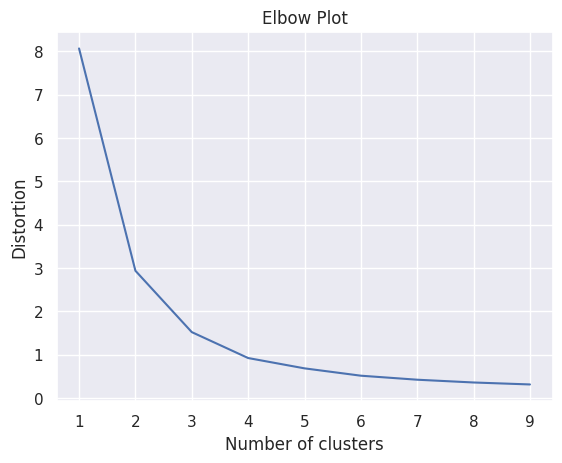
\includegraphics[width=\textwidth]{figures/tskmeans_elbow_b.png}
        \caption{Magnetic Field ($B$).}
        \label{fig:elbow_b}
    \end{subfigure}
    \hfill
    \begin{subfigure}[h]{0.48\textwidth}
        \centering
        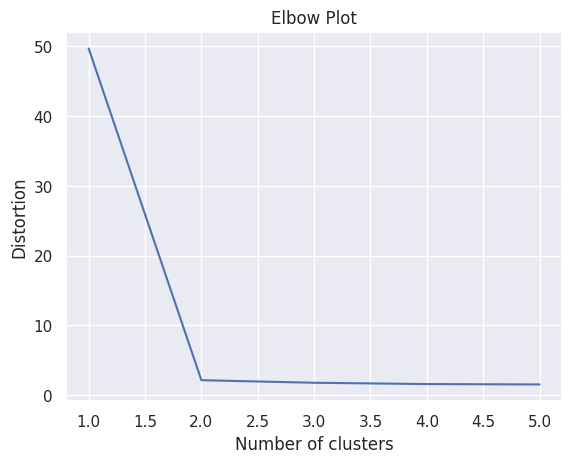
\includegraphics[width=\textwidth]{figures/tskmeans_elbow_alpha.png}
        \caption{Flux-tube inclination ($\alpha$).}
        \label{fig:elbow_alpha}
    \end{subfigure}
\end{figure}

\begin{table}[]
    \caption[Validity Scores for TimeSeriesKmeans]{Validity metrics for different TimeSeriesKMeans models obtained by varying the number of clusters.}
    \begin{subtable}[h]{0.48\textwidth}
        \centering
        \begin{tabular}{@{}cccc@{}}
            \toprule
            \textbf{K} & \textbf{S score} & \textbf{DB} & \textbf{CH} \\ \midrule
            2          & 0.524               & 0.669                   & 20376                  \\
            3          & 0.511               & 0.628                   & 25585                  \\
            4          & 0.498               & 0.606                   & 30677                  \\
            5          & 0.458               & 0.648                   & 31995                  \\
            6          & 0.449               & 0.671                   & 34394                  \\
            7          & 0.431               & 0.695                   & 35462                  \\
            8          & 0.422               & 0.712                   & 36070                  \\
            9          & 0.403               & 0.738                   & 36368                  \\ \bottomrule
        \end{tabular}
        \caption{Magnetic Field ($B$)}
        \label{tab:tskmeans_b}
    \end{subtable}
    \hfill
    \begin{subtable}[h]{0.48\textwidth}
        \centering
        \begin{tabular}{@{}cccc@{}}
            \toprule
            \textbf{K} & \textbf{S score} & \textbf{DB} & \textbf{CH} \\ \midrule
            2          & 0.865               & 0.190                   & 263222                 \\
            3          & 0.499               & 1.078                   & 160481                 \\
            4          & 0.493               & 1.089                   & 120114                 \\
            5          & 0.463               & 1.123                   & 93537                  \\
            6          & 0.480               & 1.104                   & 82431                  \\
            7          & 0.259               & 1.312                   & 82038                  \\
            8          & 0.257               & 1.306                   & 76633                  \\
            9          & 0.252               & 1.374                   & 70313                  \\ \bottomrule
            \end{tabular}
        \caption{Flux-tube inclination ($\alpha$)}
        \label{tab:tskmeans_alpha}
    \end{subtable}
\end{table}


Figure \ref{fig:elbow_b} shows the elbow test for the magnetic field variable. From this plot, it can be seen that the elbow is at $k=4$, which indicates that the optimal number of clusters is 4. However, this is not a clear elbow, as the curve is not smooth, and the elbow is not very pronounced. This indicates that the optimal number of clusters is unclear, and the results might not be very good.

The validity metrics discussed in Section \ref{sec:validity_measures} were calculated for different KMeans models obtained by varying the number of clusters to get a more precise number of clusters. The results of these tests can be seen in Table \ref{tab:tskmeans_b}. From the first three entries, it can be seen that the highest silhouette score is obtained with $K=2$, but the lowest Davies-Bouldin index is obtained with $k=4$, which also has the highest Calinski-Harabasz index of the three. This can indicate that the most appropriate number of clusters for this variable is 4.

Following the same procedure as for the magnetic field, an elbow test was conducted on the flux tube inclination variable, $\alpha$. The results of this test can be seen in Figure \ref{fig:elbow_alpha}. In contrast with the results of the previous test, this elbow is much clearer, with the elbow being at $k=2$. This indicates that the optimal number of clusters is 2.

The validity metrics (Table \ref{tab:tskmeans_alpha}) also provide a clear indication that the correct number of clusters for this variable is 2, with the highest Silhouette and Calinski-Harabasz scores being obtained with $k=2$. The Davies-Bouldin index is also the lowest for this value.


\subsection{SOM}\label{sec:som_experiments}
Following the experiments with TimeSeriesKmeans, the SOM algorithm was tested, which is also seen as a useful method for clustering high-dimension data. A Python implementation of the algorithm \cite{vettigliminisom} was tested on the same variables as the previous algorithm, $B$ and $\alpha$. Unlike KMeans, this algorithm has no tests to determine the number of clusters visually. Because of this, the number of clusters was determined by trial and error by varying the number of clusters and evaluating the results of the validity metrics (Table \ref{tab:validity_som}). The first two columns of each subtable indicate the $x$ and $y$ dimensions of the SOM map used for the clustering task. The number of clusters is obtained by multiplying these two values.

\begin{table}[]
    \caption[Validity Scores for SOM]{Validity metrics for different SOM models obtained by varying sizes of the maps ($x$ and $y$ variables).}\label{tab:validity_som}
    \begin{subtable}[h]{0.48\textwidth}
        \centering
        \begin{tabular}{@{}ccccc@{}}
            \toprule
            \textbf{x} & \textbf{y} & \textbf{S score} & \textbf{DB} & \textbf{CH} \\ \midrule
            2          & 2          & 0.500            & 0.602       & 30962   \\
            2          & 3          & 0.281            & 5.228       & 3429    \\
            3          & 2          & 0.454            & 0.660       & 35001   \\
            3          & 3          & 0.407            & 0.727       & 37133   \\ \bottomrule
            \end{tabular}
        \caption{Magnetic Field ($B$)}
        \label{tab:som_b}
    \end{subtable}
    \hfill
    \begin{subtable}[h]{0.48\textwidth}
        \centering
        \begin{tabular}{@{}ccccc@{}}
            \toprule
            \textbf{x} & \textbf{y} & \textbf{S score} & \textbf{DB} & \textbf{CH} \\ \midrule
            2          & 2          & 0.269            & 1.479       & 122195 \\
            2          & 3          & 0.004            & 1.325       & 5254    \\
            3          & 2          & 0.269            & 1.326       & 89759   \\
            3          & 3          & 0.231            & 1.426       & 66878   \\ \bottomrule
            \end{tabular}
        \caption{Flux-tube inclination ($\alpha$)}
        \label{tab:som_alpha}
    \end{subtable}
\end{table}

From looking at the results of the validity metrics for the magnetic field variable (Table \ref{tab:som_b}), it can be concluded that the highest Silhouette score and DB index are obtained with $x=2$ and $y=2$, which translate to 4 clusters. The algorithm failed to generate a proper separation for a map size of $x=2$ and $y=3$. The Calinski-Harabasz index is the highest for $x=3$ and $y=3$, which translates to 9 clusters. However, this does not indicate the correct number of clusters, as the DB index is higher than the first clustering.

The results of the validity metrics for the flux tube inclination variable (Table \ref{tab:som_alpha}) are even less clear than the previous ones. The highest Silhouette score is obtained with the first and third models. The best CH index was by far the first one. The DB index is very high for every generated model, which indicates that clustering in this variable may not be a good idea.

Overall the results from this experiment indicate that the SOM algorithm is not a good choice for clustering this dataset, as it cannot generate a clear separation between the clusters. This is especially true for the flux tube inclination variable, where the algorithm failed to generate a proper separation. The only variable where the algorithm could generate a somewhat clear separation was the magnetic field with a map of 2x2 neurons.


\subsection{PCA Clustering Approach}\label{sec:pca_clustering}
The next approach that was tested was to apply PCA to the dataset and then apply the clustering algorithms to the reduced dataset. This approach was tested on the magnetic field variable, $B[G]$, the flux tube inclination, $\alpha [deg]$, and a combination of all the input variables. 

Tests were conducted to try and find the optimal number of components that would explain the dataset. This was done by analyzing the cumulative explained variance of PCA models with different \textit{n\_components}. For $B$ and $\alpha$, about 99 \% of the variance was explained by just two components. As for the combined dataset, 98\% was explained by also two components. With this, it can be concluded that it is valid to reduce the dimensionality of this dataset to just two components. This is useful because it provides a simplified data representation while preserving most information. 

The representations for each approach can be seen in Figure \ref{fig:pca_mag_2d}. Note that the representation generated for the flux-tube indication and the joint inputs are very similar. This indicates that the flux-tube inclination variable is the one that contributes the most to the PCA.

For the clustering part, the KMeans and the AgglomerativeClustering methods of the \textit{sklearn} library were applied to each representation to determine the correct number of clusters with the same methodology as in the previous sections. 

\begin{figure}[]
    \caption[PCA applied to the different variables]{PCA applied to the different variables. (a) and (b) represent the PCAs of the magnetic field variable ($B[G]$) and the flux-tube inclination variable ($\alpha [deg]$), respectively; (c) is the PCA of all input variables combined.}
    \label{fig:pca_latent_repr}
    \begin{subfigure}[h]{0.329\textwidth}
        \centering
        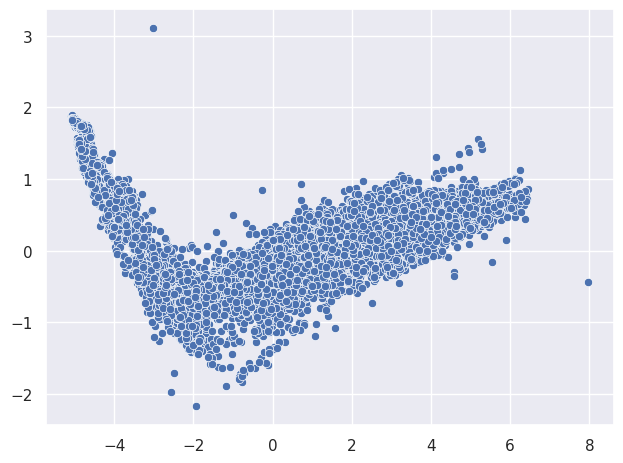
\includegraphics[width=\textwidth]{figures/mag_pca_2d.png}
        \caption{Magnetic Field ($B$).}
        \label{fig:pca_mag_2d}
    \end{subfigure}
    \hfill
    \begin{subfigure}[h]{0.329\textwidth}
        \centering
        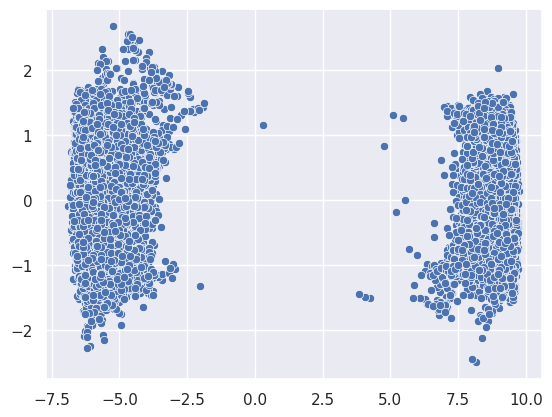
\includegraphics[width=\textwidth]{figures/alpha_pca_2d.png}
        \caption{Flux-tube inclination ($\alpha$).}
        \label{fig:pca_alpha_2d}
    \end{subfigure}
    \begin{subfigure}[h]{0.329\textwidth}
        \centering
        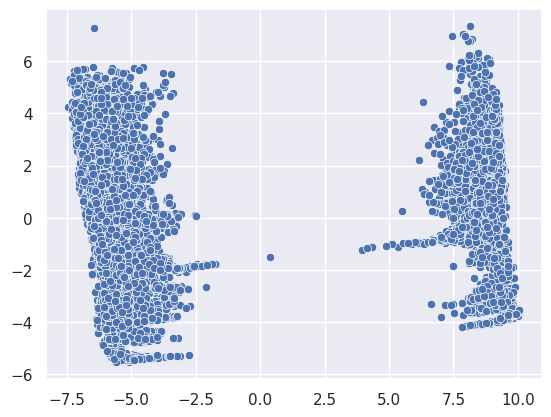
\includegraphics[width=\textwidth]{figures/pca_joint_2d.png}
        \caption{Joint Inputs ($R$, $B$ and $\alpha$).}
        \label{fig:pca_joint_2d}
    \end{subfigure}
\end{figure}

% \begin{figure}
%     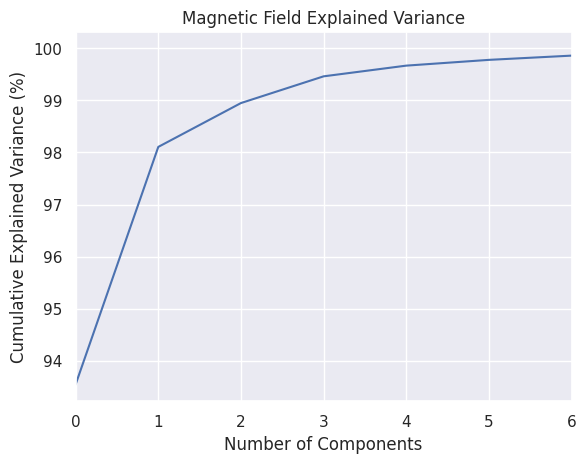
\includegraphics{figures/pca_mag_explained_variance.png}
%     \caption{Explained variance for the PCA of the magnetic field variable.}
% \end{figure}

\subsubsection{PCA of the Magnetic Field}\label{sec:pca_b}

The KMeans and the AgglomerativeClustering methods were applied to the PCA of the magnetic field variable. The results of the elbow tests for KMeans can be seen in Figure \ref{fig:pca_b_elbow}. This plot shows that the elbow is at $k=4$, indicating that the optimal number of clusters might be 4. 

\begin{figure}[h]
    \caption{KMeans Elbow test for the PCA of the magnetic field variable.}
    \label{fig:pca_b_elbow}
    \centering
    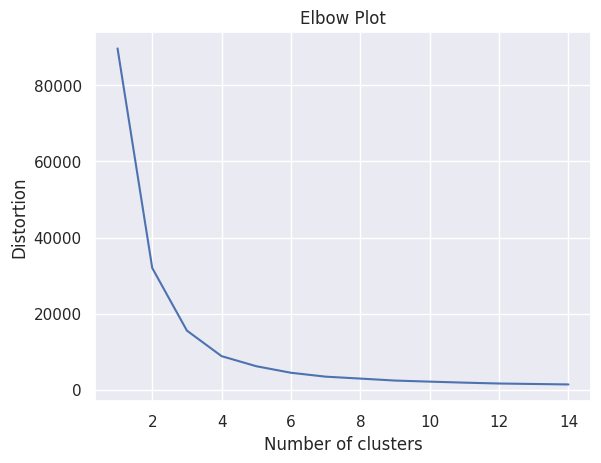
\includegraphics[width=0.6\textwidth]{figures/pca_mag_elbow_test.png}
\end{figure}

The validity measures from the previous sections were calculated for each method to get a more concrete outlook. The results of these tests can be seen in Table \ref{tab:pca_b}. For the KMeans algorithm, the highest Silhouette score is obtained with $K=2$. Still, the lowest Davies-Bouldin index is obtained with $K=4$, which also has the highest Calinski-Harabasz index of the first three results. This further confirms the results of the elbow test. 

The results of the Agglomerative method are not as clear as the previous ones. The highest silhouette score is also $K=2$, but as in KMeans, the lowest DB index was $K=4$. In addition, the CH score is much higher for the model with 4 clusters than for the $K=2$ model.

\begin{table}[]
 \caption[Validity metrics for PCA of the Magnetic Field]{Validity metrics obtained by different clustering methods on the PCA of the magnetic field variable. Various models were created for each method by varying the number of clusters, $K$.}\label{tab:pca_b}
\begin{tabular}{@{}rlrrrlrcc@{}}
\toprule
\multicolumn{1}{c}{}           &  & \multicolumn{3}{c}{\textbf{KMeans}}                                                                      &  & \multicolumn{3}{c}{\textbf{Agglomerative}}   \\ \midrule
\multicolumn{1}{c}{\textbf{K}} &  & \multicolumn{1}{c}{\textbf{S score}} & \multicolumn{1}{c}{\textbf{DB}} & \multicolumn{1}{c}{\textbf{CH}} &  & \textbf{S score} & \textbf{DB} & \textbf{CH} \\ \midrule
2                              &  & 0.538                                & 0.645                           & 21224                           &  & 0.507            & 0.669       & 17899       \\
3                              &  & 0.534                                & 0.586                           & 28086                           &  & 0.496            & 0.622       & 23868       \\
4                              &  & 0.531                                & 0.549                           & 35942                           &  & 0.502            & 0.550       & 30612       \\
5                              &  & 0.502                                & 0.579                           & 39762                           &  & 0.484            & 0.593       & 37737       \\
6                              &  & 0.494                                & 0.592                           & 44986                           &  & 0.477            & 0.585       & 40121       \\
7                              &  & 0.486                                & 0.600                           & 49233                           &  & 0.460            & 0.598       & 44158       \\
8                              &  & 0.454                                & 0.637                           & 49757                           &  & 0.436            & 0.638       & 45487       \\
9                              &  & 0.457                                & 0.636                           & 53265                           &  & 0.427            & 0.630       & 47528       \\ \bottomrule
\end{tabular}
\end{table}

With the consensus of both clustering methods, it can be concluded that the optimal number of clusters for the PCA of the magnetic field variable is 4. Interestingly, this is the same number of clusters that were obtained with the TimeSeriesKMeans algorithm in Section \ref{sec:time_series_methods} and the SOM algorithm in Section \ref{sec:som_experiments} for the magnetic field.

\subsubsection{PCA of the Flux-tube Inclination}\label{sec:pca_a}
Following the same procedure as in the previous approach, an elbow test was conducted for the KMeans model of the PCA of the flux-tube inclination variable. The results of this test can be seen in Figure \ref{fig:pca_a_elbow}. The plot indicates that the most appropriate number of clusters is 2.


\begin{figure}[]
    \caption{KMeans Elbow test for the PCA of the flux-tube inclination variable.}
    \label{fig:pca_a_elbow}
    \centering
    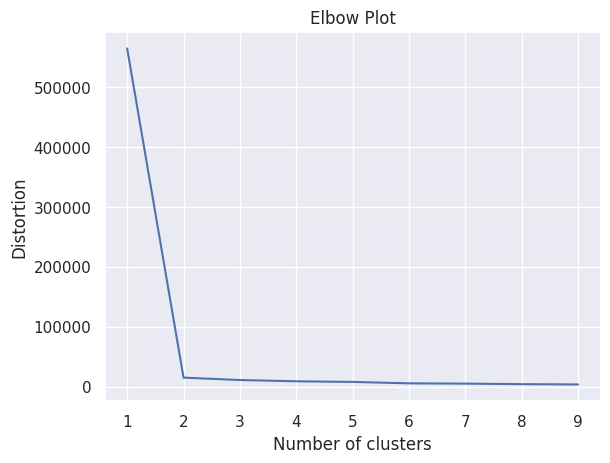
\includegraphics[width=0.6\textwidth]{figures/pca_alpha_elbow_test.png}
\end{figure}

These results are further corroborated by the validity metrics in Table \ref{tab:pca_a}. The highest Silhouette score and DB index are obtained with $K=2$, with the highest Calinski-Harabasz index of all the results. This indicates that the optimal number of clusters is 2 for both tested methods. This division occurs because the $\alpha$ variable may take negative or positive values.

\begin{table}[]
\caption[Validity metrics for PCA of the Flux-tube Inclination]{Validity metrics obtained by different clustering methods on the PCA of the flux-tube inclination variable. Various models were created for each method by varying the number of clusters, $K$.}\label{tab:pca_a}
\begin{tabular}{@{}ccccccccc@{}}
\toprule
\multicolumn{1}{l}{} & \multicolumn{1}{l}{}          & \multicolumn{3}{c}{\textbf{KMeans}}          & \multicolumn{1}{l}{\textbf{}} & \multicolumn{3}{c}{\textbf{Agglomerative}}   \\ \midrule
\textbf{K}           & \multicolumn{1}{l}{\textbf{}} & \textbf{S score} & \textbf{DB} & \textbf{CH} & \multicolumn{1}{l}{\textbf{}} & \textbf{S score} & \textbf{DB} & \textbf{CH} \\ \midrule
2                    &                               & 0.898            & 0.145       & 428761      &                               & 0.898            & 0.145       & 428761      \\
3                    &                               & 0.586            & 0.757       & 294424      &                               & 0.574            & 0.782       & 287595      \\
4                    &                               & 0.593            & 0.662       & 243422      &                               & 0.378            & 1.022       & 239082      \\
5                    &                               & 0.583            & 0.713       & 207238      &                               & 0.354            & 0.955       & 219099      \\
6                    &                               & 0.400            & 0.887       & 237197      &                               & 0.359            & 0.924       & 215351      \\
7                    &                               & 0.392            & 0.917       & 216689      &                               & 0.360            & 0.900       & 211272      \\
8                    &                               & 0.391            & 0.875       & 225758      &                               & 0.338            & 0.906       & 199083      \\
9                    &                               & 0.381            & 0.901       & 223637      &                               & 0.336            & 0.890       & 189224      \\ \bottomrule
\end{tabular}
\end{table}

\subsubsection{PCA of the Joint Inputs}\label{sec:pca_joint}
The PCA was applied to the joint inputs, $R$, $B$ and $\alpha$ in this next approach to capture the most relevant features of the input variables, as they would later be used in the prediction task. The results of the elbow test for the KMeans algorithm can be seen in Figure \ref{fig:pca_joint_elbow}. It is difficult to determine the optimal number of clusters from this plot. Possible "elbows" include the ones at $K=3$ and $K=6$.

\begin{figure}[h]
    \caption{KMeans Elbow test for the PCA of the joint inputs.}
    \label{fig:pca_joint_elbow}
    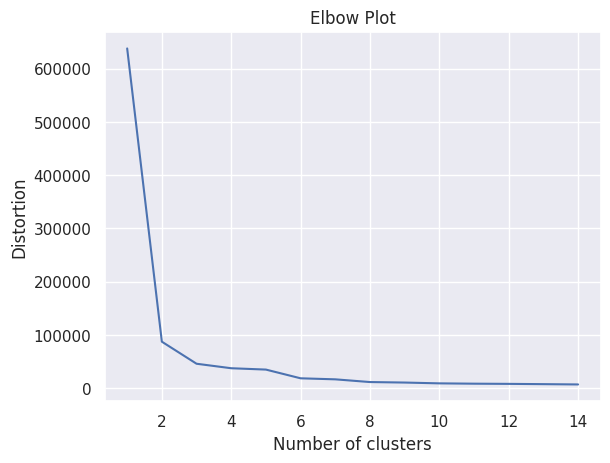
\includegraphics[width=0.6\textwidth]{figures/pca_joint_elbow_test.png}
\end{figure}

\begin{table}[h]
 \caption[Validity metrics for PCA of the Joint Inputs]{Validity metrics obtained by different clustering methods on the PCA of the joint inputs. Various models were created for each method by varying the number of clusters, $K$.}\label{tab:pca_joint}
\begin{tabular}{@{}lllrclccc@{}}
\toprule
           &           & \multicolumn{3}{c}{\textbf{KMeans}}          & \textbf{} & \multicolumn{3}{c}{\textbf{Agglomerative}}   \\ \midrule
\textbf{K} & \textbf{} & \textbf{S score} & \textbf{DB} & \textbf{CH} & \textbf{} & \textbf{S score} & \textbf{DB} & \textbf{CH} \\ \midrule
2          &           & 0.777            & 0.326       & 74261       &           & 0.777            & 0.326       & 74261       \\
3          &           & 0.647            & 0.494       & 75974       &           & 0.625            & 0.503       & 70716       \\
4          &           & 0.605            & 0.567       & 62966       &           & 0.544            & 0.564       & 72768       \\
5          &           & 0.553            & 0.698       & 50851       &           & 0.510            & 0.620       & 84236       \\
6          &           & 0.471            & 0.714       & 78768       &           & 0.464            & 0.704       & 86339       \\
7          &           & 0.465            & 0.747       & 73566       &           & 0.427            & 0.789       & 83135       \\
8          &           & 0.438            & 0.777       & 91850       &           & 0.396            & 0.819       & 82333       \\
9          &           & 0.435            & 0.786       & 87596       &           & 0.382            & 0.858       & 82094       \\ \bottomrule
\end{tabular}
\end{table}

To draw better conclusions, the validity metrics were calculated for each method. The results of these tests can be seen in Table \ref{tab:pca_joint}. For the KMeans algorithm, the highest Silhouette score and DB index are from $K=2$. This conflicts with the results of the elbow test, which indicated that the optimal number of clusters was 3 or 6. The highest CH index of the three is with $K=6$, but this model has the worst Silhouette and DB scores. At first glance, the optimal number of clusters would be 2 for the KMeans algorithm.

Next, for the Agglomerative method, the best silhouette score is from $K=2$ with the same results as the previous method. This is because both algorithms generate the same clear division of the dataset into two clusters that can easily be construed from Figure \ref{fig:pca_joint_2d}. The remaining validity metrics are also very similar to the ones obtained with the KMeans algorithm. However, the clusters generated by the Agglomerative method for $K=3$ had a smaller CH score than the ones for $K=2$. This might indicate that this method's best number of clusters is 2.

% Please add the following required packages to your document preamble:
% \usepackage{booktabs}


\subsection{t-SNE Clustering Approach}\label{sec:tsne_clustering}
The last tested approach was to apply t-SNE to the dataset and then apply the clustering algorithms to the reduced dataset. As with the previous approach, this one was tested on the magnetic field variable, $B[G]$, the flux tube inclination, $\alpha [deg]$, and lastly, on a combination of all the input variables. The embedded 2D representations obtained from the t-SNE algorithm can be seen in Figure \ref{fig:tsne_2d}. Looking at the first two, it can be concluded that the clustering task will be more complicated than the PCA representations.

\begin{figure}[h]
    \caption[t-SNE applied to the different variables]{t-SNE applied to the different variables. (a) and (b) represent the t-SNE of the magnetic field variable ($B[G]$) and the flux-tube inclination variable ($\alpha [deg]$), respectively; (c) is the t-SNE of all input variables combined.}
    \label{fig:tsne_2d}
    \begin{subfigure}[h]{0.329\textwidth}
        \centering
        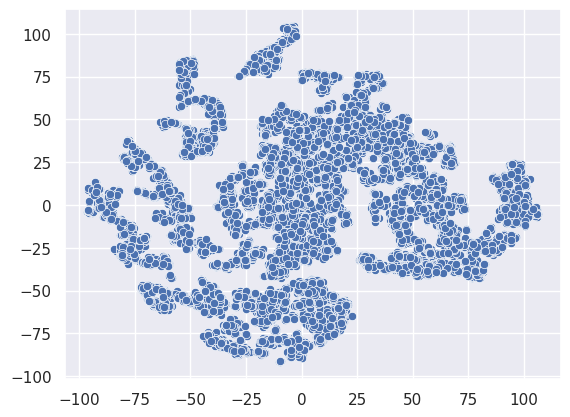
\includegraphics[width=\textwidth]{figures/tsne_mag_2d.png}
        \caption{Magnetic Field ($B$).}
        \label{fig:tsne_mag_2d}
    \end{subfigure}
    \hfill
    \begin{subfigure}[h]{0.329\textwidth}
        \centering
        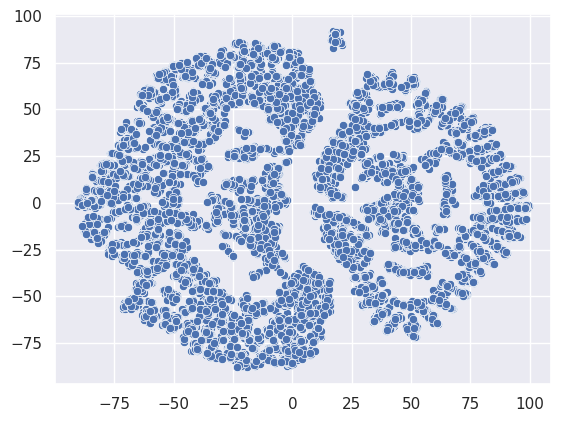
\includegraphics[width=\textwidth]{figures/tsne_alpha_2d.png}
        \caption{Flux-tube inclination ($\alpha$).}
        \label{fig:tsne_alpha_2d}
    \end{subfigure}
    \begin{subfigure}[h]{0.329\textwidth}
        \centering
        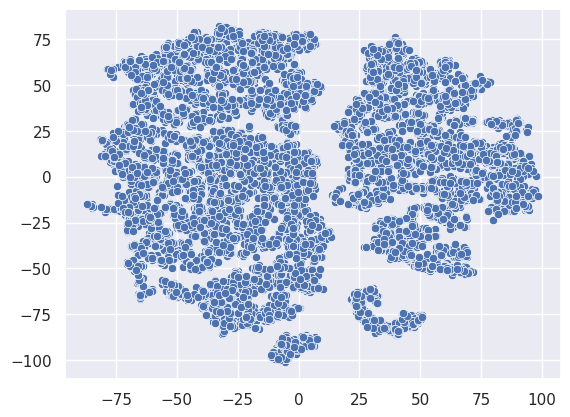
\includegraphics[width=\textwidth]{figures/tsne_joint_2d.png}
        \caption{Joint Inputs ($R$, $B$ and $\alpha$).}
        \label{fig:tsne_joint_2d}
    \end{subfigure}
\end{figure}

As in the previous section, each representation was subjected to the KMeans and Agglomerative clustering algorithms from the \textit{sklearn} library. The same validity metrics were calculated to determine what number of clusters would generate the best clustering.

\subsubsection{t-SNE of the Magnetic Field}\label{sec:tsne_b}
The elbow test for the magnetic field variable was inconclusive, as the elbow was unclear. Possible values could be with 4 or 6 clusters. The highest Silhouette score is obtained with $K=2$, but the lowest Davies-Bouldin index is obtained with $K=4$, with the highest Calinski-Harabasz index of the first three results. 

% \begin{figure}
%     \caption{KMeans Elbow test for the t-SNE of the magnetic field variable.}
%     \label{fig:tsne_b_elbow}
%     \centering
%     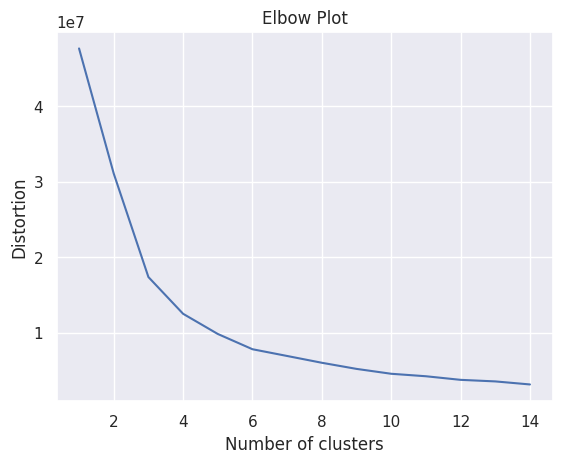
\includegraphics[width=0.6\textwidth]{figures/tsne_mag_elbow_test.png}
% \end{figure}

The validity metrics from Table \ref{tab:tsne_b} show a clear candidate for the KMeans method at $K=6$, which has the best scores of every other model. This disambiguates the results of the elbow test conducted previously. For the Agglomerative clustering method, the results aren't as pronounced. The best silhouette and DB scores were obtained for 6 clusters. Despite the CH index not being as higher as the rest, there is not much variation of this metric above 5 clusters. The results of this test indicate that the optimal number of clusters is 6 for both clustering methods.

% Please add the following required packages to your document preamble:
% \usepackage{booktabs}
\begin{table}[]
\caption[Validity metrics for t-SNE of the Magnetic Field]{Validity metrics obtained by different clustering methods on the t-SNE of the magnetic field variable. Various models were created for each method by varying the number of clusters, $K$.}\label{tab:tsne_b}
\begin{tabular}{@{}ccccccccc@{}}
\toprule
\multicolumn{1}{l}{} & \multicolumn{1}{l}{} & \multicolumn{3}{c}{\textbf{KMeans}}          & \multicolumn{1}{l}{} & \multicolumn{3}{c}{\textbf{Agglomerative}}   \\ \midrule
\textbf{K}           & \textbf{}            & \textbf{S score} & \textbf{DB} & \textbf{CH} & \textbf{}            & \textbf{S score} & \textbf{DB} & \textbf{CH} \\ \midrule
2                    &                      & 0.323            & 1.265       & 6275.825    &                      & 0.361            & 1.141       & 7475.524    \\
3                    &                      & 0.404            & 0.863       & 10259.411   &                      & 0.349            & 0.883       & 7335.993    \\
4                    &                      & 0.409            & 0.838       & 11029.298   &                      & 0.386            & 0.848       & 9553.107    \\
5                    &                      & 0.400            & 0.867       & 11319.886   &                      & 0.387            & 0.853       & 10085.435   \\
6                    &                      & 0.424            & 0.756       & 12010.235   &                      & 0.390            & 0.777       & 10395.708   \\
7                    &                      & 0.406            & 0.831       & 11557.172   &                      & 0.358            & 0.842       & 10453.778   \\
8                    &                      & 0.402            & 0.798       & 11639.116   &                      & 0.346            & 0.823       & 10364.565   \\
9                    &                      & 0.397            & 0.792       & 11998.942   &                      & 0.357            & 0.827       & 10653.976   \\
10                   &                      & 0.403            & 0.785       & 12363.613   &                      & 0.373            & 0.820       & 11237.525   \\ \bottomrule
\end{tabular}
\end{table}

\subsubsection{t-SNE of the Flux-tube Inclination}\label{sec:tsne_a}
In line with the results from the experiments on the magnetic field, the elbow test for the $\alpha$ variable is also difficult to interpret. The elbow is not clear enough to be able to reach an estimation.

\begin{table}[]
\caption[Validity metrics for t-SNE of the Flux-tube Inclination]{Validity metrics obtained by different clustering methods on the t-SNE of the flux-tube inclination variable. Various models were created for each method by varying the number of clusters, $K$.}\label{tab:tsne_a}
\begin{tabular}{@{}ccccccccc@{}}
\toprule
           &  & \multicolumn{3}{c}{\textbf{KMeans}}          & \textbf{} & \multicolumn{3}{c}{\textbf{Agglomerative}}   \\ \midrule
\textbf{K} &  & \textbf{S score} & \textbf{DB} & \textbf{CH} & \textbf{} & \textbf{S score} & \textbf{DB} & \textbf{CH} \\ \midrule
2          &  & 0.367            & 1.142       & 7613        &           & 0.343            & 1.112       & 6787        \\
3          &  & 0.410            & 0.803       & 10814       &           & 0.385            & 0.864       & 9815        \\
4          &  & 0.389            & 0.817       & 11185       &           & 0.350            & 0.887       & 8899        \\
5          &  & 0.382            & 0.877       & 11611       &           & 0.336            & 0.945       & 9269        \\
6          &  & 0.365            & 0.866       & 11396       &           & 0.366            & 0.867       & 9925        \\
7          &  & 0.396            & 0.779       & 12086       &           & 0.351            & 0.861       & 10223       \\
8          &  & 0.394            & 0.754       & 12678       &           & 0.338            & 0.799       & 10276       \\
9          &  & 0.395            & 0.776       & 12365       &           & 0.325            & 0.785       & 10429       \\
10         &  & 0.398            & 0.789       & 13223       &           & 0.341            & 0.853       & 10870       \\ \bottomrule
\end{tabular}
\end{table}

The validity metrics in Table \ref{tab:tsne_a} also fail to indicate the optimal number of clusters for the KMeans algorithm. This can be because the algorithm is not suited to handle this representation, as it is very complex. The same can be said of the Agglomerative method, with all entries having very similar silhouette scores. A comparison of both DB and CH scores indicates that the number of clusters for both methods can be 8 or 9, but there is no clear indication of which is best.

% Please add the following required packages to your document preamble:
% \usepackage{booktabs}

\subsubsection{t-SNE of the Joint Inputs}\label{sec:tsne_joint}
Contrary to the other two variables, the elbow test for the joint inputs was very clear with an elbow at $K=3$, indicating that the optimal number of clusters is 3. This is also corroborated by the validity metrics in Table \ref{tab:tsne_joint}. For the KMeans algorithm, the highest Silhouette score and DB index are $K=2$, which also has the highest Calinski-Harabasz index of the first three results. Another possible division would be 7 clusters because of the similar silhouette and DB scores and a higher CH score. 

% \begin{figure}[]
%     \caption{KMeans Elbow test for the t-SNE of the joint inputs.}
%     \label{fig:tsne_joint_elbow}
%     \centering
%     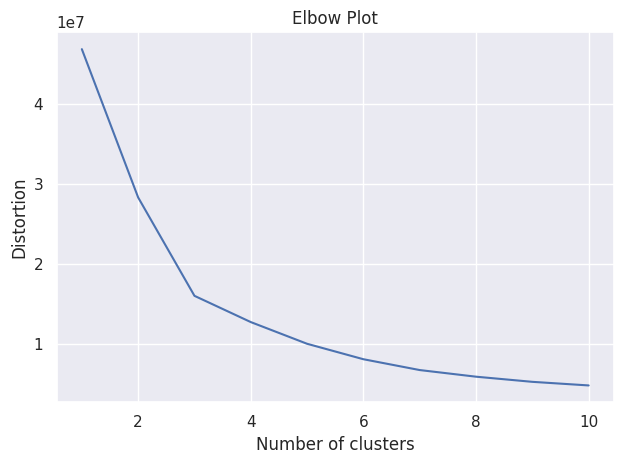
\includegraphics[width=0.6\textwidth]{figures/tsne_joint_elbow_test.png}
% \end{figure}

For the Agglomerative method, the most appropriate number of clusters is 3. Despite having a worse DB index than $K=4$, the silhouette and CH scores are better. This indicates that the optimal number of clusters is 3 for both clustering methods.


% Please add the following required packages to your document preamble:
% \usepackage{booktabs}
\begin{table}[]
\caption[Validity metrics for t-SNE of the Joint Inputs]{Validity metrics obtained by different clustering methods on the t-SNE of the joint inputs. Various models were created for each method by varying the number of clusters, $K$.}\label{tab:tsne_joint}
\begin{tabular}{@{}ccccccccc@{}}
\toprule
\multicolumn{1}{l}{\textbf{}} & \multicolumn{1}{l}{\textbf{}} & \multicolumn{3}{c}{\textbf{KMeans}}          & \multicolumn{1}{l}{\textbf{}} & \multicolumn{3}{c}{\textbf{Agglomerative}}   \\ \midrule
\textbf{K}                    & \textbf{}                     & \textbf{S score} & \textbf{DB} & \textbf{CH} & \textbf{}                     & \textbf{S score} & \textbf{DB} & \textbf{CH} \\ \midrule
2                             &                               & 0.383            & 1.067       & 7701        &                               & 0.328            & 1.068       & 5684        \\
3                             &                               & 0.430            & 0.791       & 11317       &                               & 0.400            & 0.851       & 10083       \\
4                             &                               & 0.384            & 0.829       & 10493       &                               & 0.370            & 0.790       & 9549        \\
5                             &                               & 0.370            & 0.918       & 10792       &                               & 0.341            & 0.902       & 9797        \\
6                             &                               & 0.391            & 0.856       & 11249       &                               & 0.330            & 0.972       & 9609        \\
7                             &                               & 0.399            & 0.798       & 11645       &                               & 0.319            & 1.015       & 9572        \\
8                             &                               & 0.385            & 0.806       & 11612       &                               & 0.328            & 0.941       & 9924        \\
9                             &                               & 0.377            & 0.850       & 11576       &                               & 0.341            & 0.894       & 10287       \\
10                            &                               & 0.379            & 0.820       & 11369       &                               & 0.337            & 0.888       & 10364       \\ \bottomrule
\end{tabular}
\end{table}

\subsection{DBSCAN Experiments}\label{sec:dbscan_pca_exp}
Additional experiments were carried out with the DBSCAN clustering method on both PCA and t-SNE representations. This algorithm was chosen because it can perform the clustering task and detect anomalies simultaneously. 

\begin{figure}[]
    \caption[DBSCAN results on PCA of the magnetic field]{DBSCAN results on PCA of $B [G]$. (a) DBSCAN clustering of the PCA of the magnetic field, $B [G]$; (b) magnetic field lines separated by clusters (-1 is the outliers).}
    \begin{subfigure}[h]{0.37\textwidth}
        \centering
        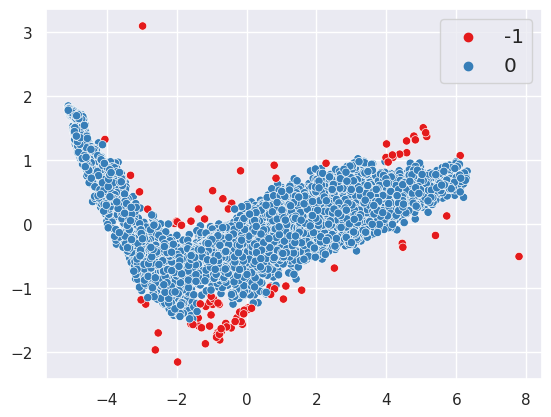
\includegraphics[width=\textwidth]{figures/dbscan_mag.png}
        \caption{DBSCAN clustering}
        \label{fig:dbscan_mag_clusters}
    \end{subfigure}
    \hfill
    \begin{subfigure}[h]{0.62\textwidth}
        \centering
        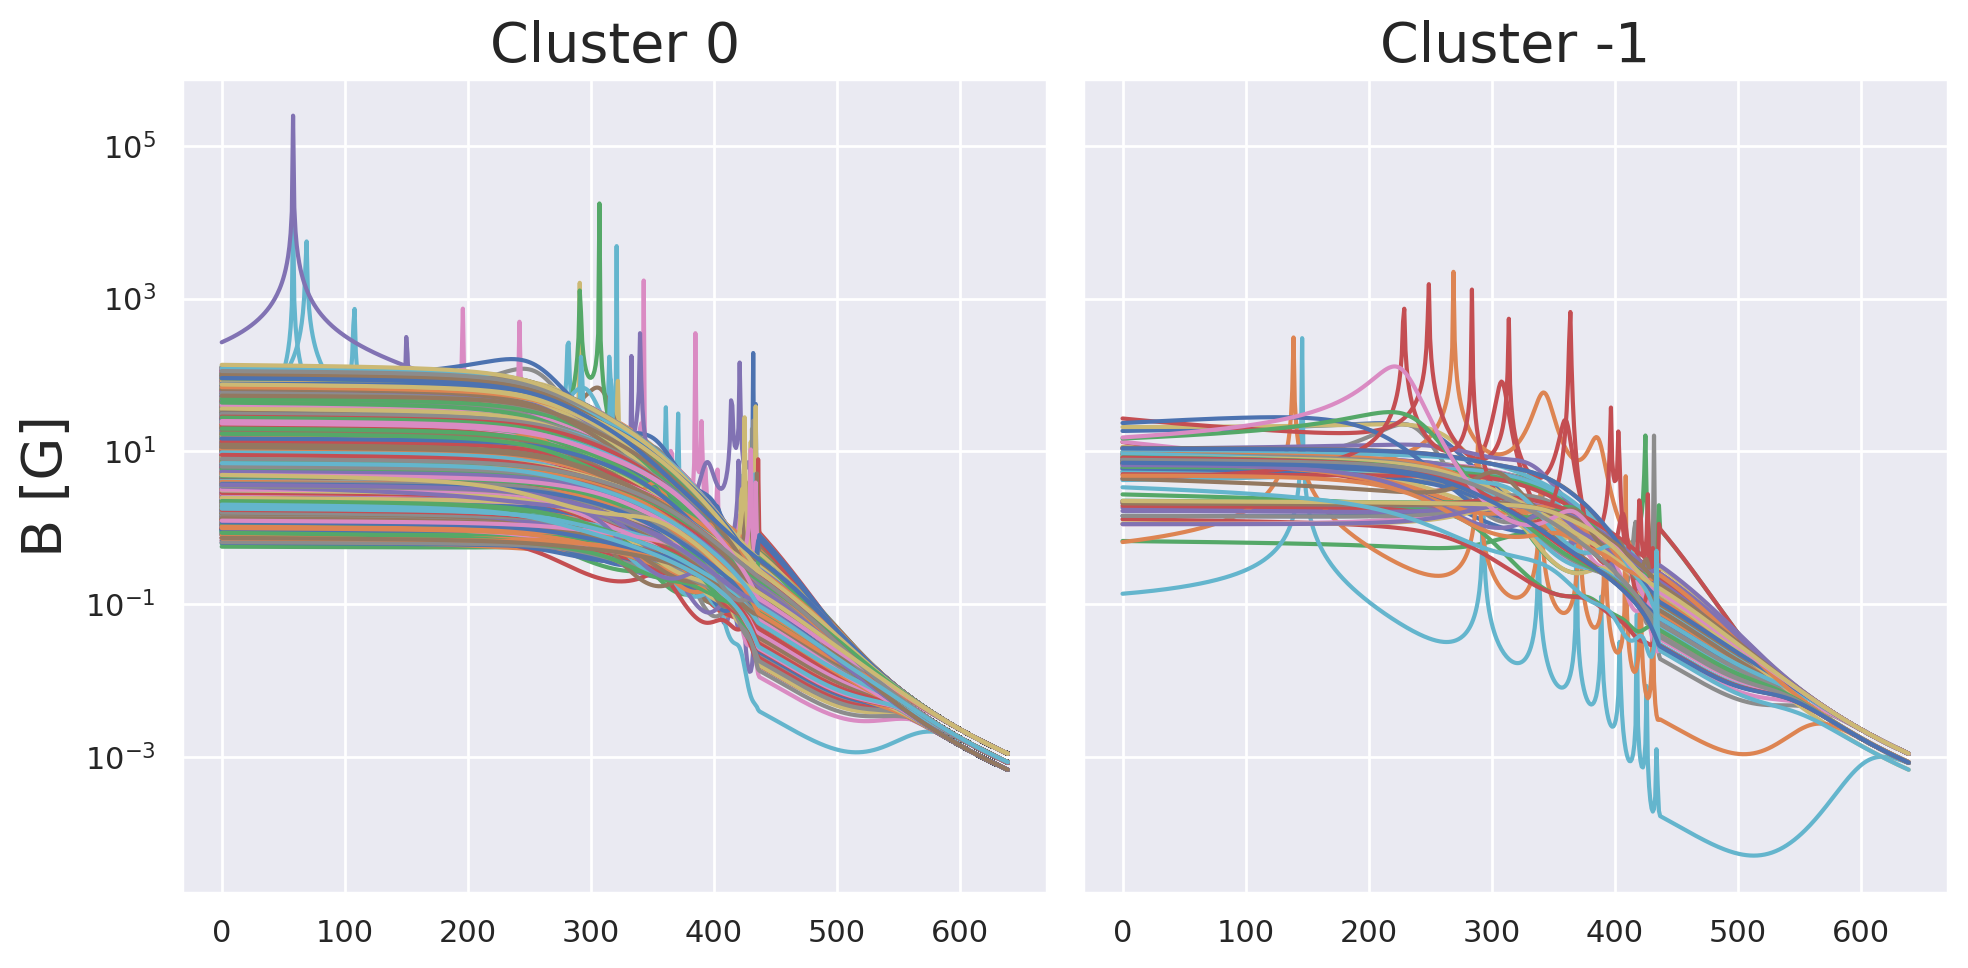
\includegraphics[width=\textwidth]{figures/dbscan_cluster_repr.png}
        \caption{}% TODO
        \label{fig:mag_dbscan_cluster_real}
    \end{subfigure}
\end{figure}

The tests were carried out in each of the representations from Sections \ref{sec:pca_clustering} and \ref{sec:tsne_clustering}. The only experiment that yielded somewhat good results was when DBSCAN was applied to the PCA of the magnetic field variable. 

Figure \ref{fig:dbscan_mag_clusters} shows the clustering obtained for this method, and Figure \ref{fig:mag_dbscan_cluster_real} the separation of the magnetic field lines per cluster. From there, it can be concluded that this method can serve as a basic anomaly detection approach. The method can detect some anomalies in the magnetic field variable (cluster -1); however, many anomalous lines remain in the final dataset (presented in cluster 0).

The results from these experiments might have been hindered by using the \textit{QuantileTransformer}, which tends to mitigate the effects of outliers. More appropriate scalers for outlier detection tasks were tested to try and improve the test outcome. Due to several extreme values, these failed to produce valid representations that DBSCAN could use.

\section{ML Experiments}\label{sec:clustering_ml_experiments}
Following the mostly exploratory clustering experiments, the next step was to apply the clustering algorithms to the dataset and then use the resulting clusters to train different machine learning models. This experiment aimed to determine if models trained on clusters generated by different algorithms could produce better predictions than models trained on the entire dataset. 

The reasoning is that by grouping similar data points, the models could learn more specific patterns for each cluster. This is especially useful in this context as the data is very dispersed, and the resulting models would converge to the mean of the dataset. % TODO referenciar Filipa

Due to the difficulty in selecting the most appropriate clustering, a grid-search-based approach was followed for this task. Several clusterings, $C$, were generated for each method described in the previous sections by varying the number of clusters, $K$. The same clustering parameters from the previous experiments were used for consistency because they were chosen to be the most appropriate for each method and the dataset at hand.

Then, an ML model, $M_i$, was trained for each of the generated clusterings, $C_i$, was trained for each cluster, $C_{ij}$, where $i$ is the ith clustering and $j$ is the jth cluster of $C$. Each model, $M_i$, is trained with the same methodology as in \cite{barros_InitialConditionEstimation_}. This time, instead of training a single model for the entire dataset, a model was trained for each cluster, $C_{ij}$. 

Following the methodology in Barros \cite{barros_InitialConditionEstimation_}, the same validation files were extracted from the training dataset for later use in the MULTI-VP tests. For each cluster, $C_{ij}$, a train test split of 85/15 \% was done to obtain training and testing datasets. The training dataset was then used to train the models $M_{ij}$, and the testing dataset was later used to evaluate the models in terms of performance. In the next step, a hyper-tuning random search model from the \textit{keras} \cite{chollet2015keras} library was employed to find the best hyper-parameters for $M_{ij}$, based on the best test MSE loss. Finally, the best model was saved for later use in the MULTI-VP experiments. 

The generated models were saved along with their statistics and the hyper-parameters used. The results of the MULTI-VP experiments can be seen in Section \ref{sec:clustering_ml_results}.

\subsection{Clustering ML Results}\label{sec:clustering_ml_results}
The results from the above-mentioned experiments are presented in Table \ref{tab:clustering_ml_results}. Only the top 10 results based on MSE loss measured on the testing dataset are shown. The models are sorted based on the average MSE loss in each experiment. This is obtained by averaging the MSE loss of each model, $M_{ij}$, for each cluster, $C_{ij}$, of each clustering, $C_i$. The models are sorted from lowest to highest average loss. The first column shows the model ID, which briefly characterizes the model, the dimensionality reduction method, the variables used in the clustering, the clustering method, the number of clusters, $K$, and the models' average loss and standard deviation.


\begin{table}[]
    \caption[Results of the Clustering ML Experiments]{Results of the Clustering ML Experiments. The table shows the ten best models based on the average MSE loss. The models are sorted by the average loss, from lowest to highest. The columns show the model ID, the dimensionality reduction method, the variables used, the clustering method, the number of clusters, $K$, the average loss of the models, the standard deviation of the loss and the sum of the loss and the standard deviation.}\label{tab:clustering_ml_results}
    \begin{tabular}{@{}cccccrr@{}}
    \toprule
    \textbf{Model ID}     & \textbf{Dim. Reduct.} & \textbf{Variable} & \textbf{Method} & \textbf{K} & \multicolumn{1}{c}{\textbf{Avg. Loss}} & \multicolumn{1}{c}{\textbf{std Loss}} \\ \midrule
    tsne\_agg\_2          & TSNE                  & Joint             & Agglom.         & 2          & 0.0108                                 & 0.0058                                \\
    pca\_kmeans\_2        & PCA                   & Joint             & KMeans          & 2          & 0.0113                                 & 0.0016                                \\
    pca\_kmeans\_3        & PCA                   & Joint             & KMeans          & 3          & 0.0119                                 & 0.0037                                \\
    pca\_agg\_2           & PCA                   & Joint             & Agglom.         & 2          & 0.0125                                 & 0.0012                                \\
    tsne\_kmeans\_mag\_3  & TSNE                  & Mag. Field        & KMeans          & 3          & 0.0125                                 & 0.0085                                \\
    tsne\_agg\_8          & TSNE                  & Joint             & Agglom.         & 8          & 0.0127                                 & 0.0077                                \\
    tsne\_agg\_alpha\_2   & TSNE                  & Alpha             & Agglom.         & 2          & 0.0129                                 & 0.0003                                \\
    pca\_kmeans\_alpha\_2 & PCA                   & Alpha             & KMeans          & 2          & 0.0130                                 & 0.0009                                \\
    tsne\_agg\_3          & TSNE                  & Joint             & Agglom.         & 3          & 0.0132                                 & 0.0093                                \\
    tsne\_agg\_mag\_3     & TSNE                  & Joint             & Agglom.         & 3          & 0.0132                                 & 0.0090                                \\ \bottomrule
    \end{tabular}
\end{table}


The experimental results (Table \ref{tab:clustering_ml_results}) show that the best models were obtained with the clusterings of the TSNE joint inputs. These divisions were obtained by running the Agglomerative Clustering method with $K=2$. A closer look at the standard deviation of this model shows that it is the highest of the top 3 models, indicating a large disparity between the losses of both models. 

% \begin{figure}
%     \caption{Visualization of the clusters obtained with the TSNE of the joint inputs.}
%     \label{fig:tsne_joint_kmeans_2}
%     \centering
%     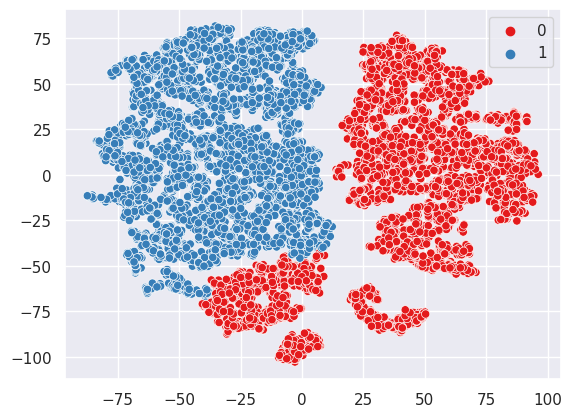
\includegraphics[width=0.6\textwidth]{figures/tsne_joint_kmeans_2.png}
% \end{figure}

A more in-depth analysis of this outcome with the validity methods from Table \ref{tab:tsne_joint} contradicts the results from this experiment. Despite it having the lowest loss of all the entries, the clustering quality was subpar for this instance. The inappropriate clustering of the dataset might be the reason for the high standard deviation of the models, as the data was not grouped correctly. A visualization of the clustering from this method is presented in Appendix \ref{fig_a:tsne_joint_kmeans_2}.


\begin{figure}[]
    \caption[Top clustering results for the KMeans applied to the PCA of the joint inputs.]{Top clustering results for the KMeans applied to the PCA of the joint inputs. Clusters were obtained with the KMeans algorithm on the PCA of the joint inputs with $K=2$ on the left and $K=3$ on the right.}
    \label{fig:pca_joint_kmeans_results}
    \begin{subfigure}[h]{0.49\textwidth}
        \centering
        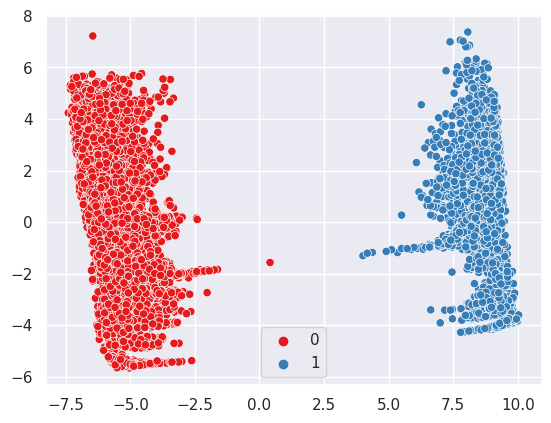
\includegraphics[width=\textwidth]{figures/pca_joint_kmeans_2.png}
        \caption{2 clusters}
        \label{fig:pca_joint_kmeans_2}
        % \label{fig:tsne_mag_2d}
    \end{subfigure}
    \hfill
    \begin{subfigure}[h]{0.49\textwidth}
        \centering
        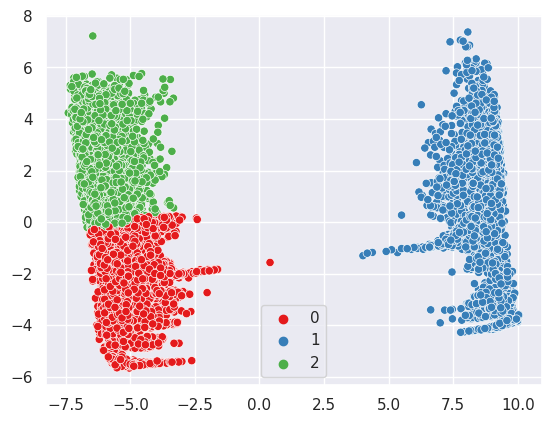
\includegraphics[width=\textwidth]{figures/pca_joint_kmeans_3.png}
        \caption{3 clusters}
        \label{fig:pca_joint_kmeans_3}
    \end{subfigure}
\end{figure}

The second-best results were obtained with the KMeans clustering of the PCA of the joint inputs. The standard deviation of this model is the lowest of the top three models, which indicates that the losses of the models are very similar. Despite the average loss not being as low as with the first method, it is still not far off. An analysis of the clustering results from the previous section (Table \ref{tab:pca_joint}) shows that the clustering quality was also very good. This indicates that the models could learn the patterns of the clusters and that the clustering was appropriate for the dataset. A visualization of the clusters in Figure \ref{fig:pca_joint_kmeans_2} also corroborates this by dividing the dataset into two clusters.

The next best method was delined by training a model for each cluster of the same representation as the previous one but with $K=3$. Although the average loss is higher than the previous two, the standard deviation is also very low, which indicates that the losses of the models are similar, in contrast with the disparity of the models from the second experiment. The clusters for this experiment can be seen in Figure \ref{fig:pca_joint_kmeans_3}.

These two experiments serve as the principal contenders for the best models. The results from the previous section were further analyzed to disambiguate the results. As was already concluded, in section \ref{sec:pca_joint}, the elbow test (Figure \ref{fig:pca_joint_elbow}) produced a clear spike at $K=2$; however, the elbow might be at $K=3$. The validity metrics (Table \ref{tab:pca_joint}) for the KMeans clustering indicate that the best separation is with two clusters just from the silhouette score and DH index. Despite this, the CH index is slightly lower than with $K=3$. 

Taking all these factors into consideration, the models that were selected were the ones obtained with the KMeans clustering with $K=3$. In addition to the reasons mentioned above, this clustering provides an equal division of the dataset, in contrast with the other clustering with $K=2$, which has a very large and small cluster.

An analysis of the remaining results shows that no model trained on other clustering algorithms produced better results than the ones obtained with the PCA and TSNE. Most of the top results (7 out of 10) were obtained with the clusterings of the joint input variables. In addition, every clustering was obtained by dimensionality reductions of the original dataset. This might indicate that the clustering methods trained on the original dataset could not find the best clusters for the dataset. 

\clearpage
\subsection{MULTI-VP Results}\label{sec:clustering_mulivp_results}
This section presents the results of the MULTI-VP simulation with the initial conditions of the developed prediction models.

\begin{figure}[h]
    \caption[Clustering MULTI-VP error comparison for N]{Abscissa wise estimate error comparison of $n [cm^3]$. (a) comparison of the baseline model and initial expert estimates; (b) comparison of the estimates with the clustering approach and expert predictions.}
    \begin{subfigure}[]{0.48\textwidth}
        \centering
        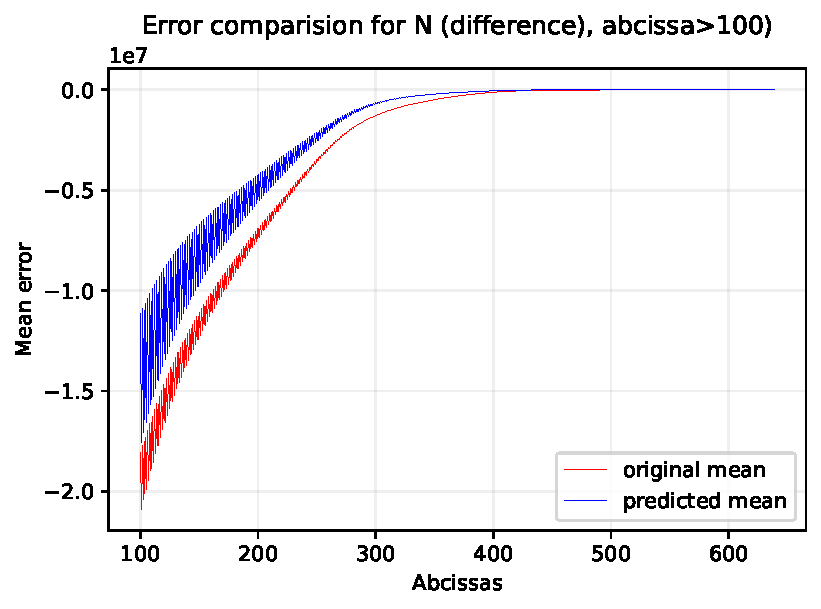
\includegraphics[width=\textwidth]{figures/N_error_comparison_after100_filipa.pdf}
        \caption{Baseline model}
        \label{fig:n_error_filipa}
    \end{subfigure}
    \hfill
    \begin{subfigure}[]{0.48\textwidth}
        \centering
        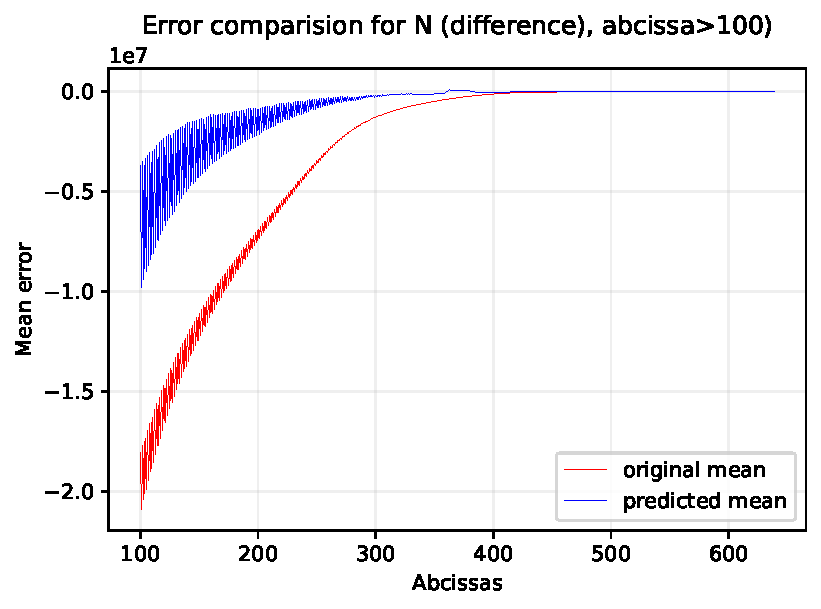
\includegraphics[width=\textwidth]{figures/N_error_comparison_after100_clusters.pdf}
        \caption{Clustering models}
        \label{fig:n_error_cluster_no_overfit}
    \end{subfigure}
\end{figure}

Figure \ref{fig:n_error_filipa} shows the abscissa-wise mean error comparison on the $n [cm^3]$ variable. This chart displays the difference between the estimates provided as input for the simulation and its final estimates. The red line displays the error between the initial expert guesses and the final prediction. Similarly, the blue shows the difference between the outputs of the prediction model and the final estimates of the simulation. The results prove that the initial estimates generated by the prediction model in \cite{barros_InitialConditionEstimation_} are closer to the expected result of the simulation than the expert estimates. 

The results obtained with the three cluster models (Figure \ref{fig:v_error_cluster}) show a significant decrease in the mean error of the predictions (blue) when compared to the original estimates (red). In addition, the mean error of the predictions from these new models is lower than that obtained with the baseline model. This shows that the approach resulted in $v [cm³]$ values closer to the final MULTI-VP simulation.


\begin{figure}[]
    \caption[Clustering MULTI-VP error comparison for V]{Abscissa wise estimate error comparison of $v [km/s]$. (a) comparison of the baseline model and initial expert estimates; (b) comparison of the estimates with the clustering approach and expert predictions.}
    \begin{subfigure}[]{0.48\textwidth}
        \centering
        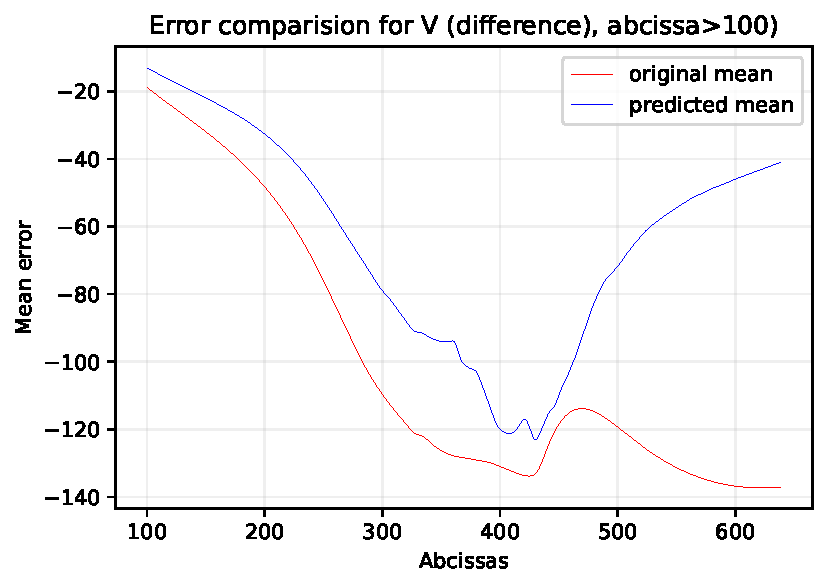
\includegraphics[width=\textwidth]{figures/V_error_comparison_after100_filipa.pdf}
        \caption{Baseline model}
        \label{fig:v_error_filipa}
    \end{subfigure}
    \hfill
    \begin{subfigure}[]{0.48\textwidth}
        \centering
        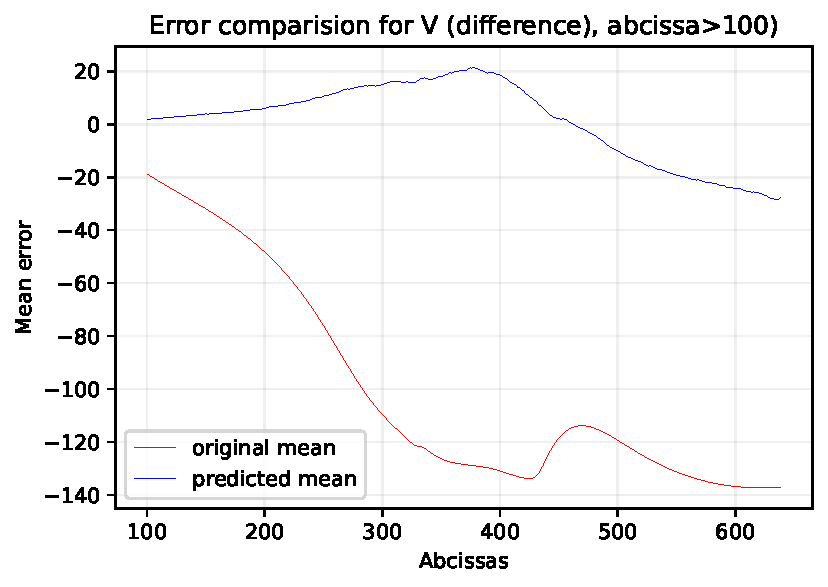
\includegraphics[width=\textwidth]{figures/V_error_comparison_after100_clusters.pdf}
        \caption{Clustering models}
        \label{fig:v_error_cluster}
    \end{subfigure}
\end{figure}

For the $v [km/s]$, the baseline model (Figure \ref{fig:v_error_filipa}) shows similar mean error for its predictions and the original expert estimates. In contrast, the cluster-based approach predicted values of $v [k/m]$ closer to the final MULTI-VP simulation, as can be seen by the significantly lower mean error for these when compared to the expert estimates.

\begin{figure}[]
    \caption[Clustering MULTI-VP error comparison for T]{Abscissa wise estimate error comparison of $T [MK]$. (a) comparison of the baseline model and initial expert estimates; (b) comparison of the estimates with the clustering approach and expert predictions.}
    \begin{subfigure}[]{0.48\textwidth}
        \centering
        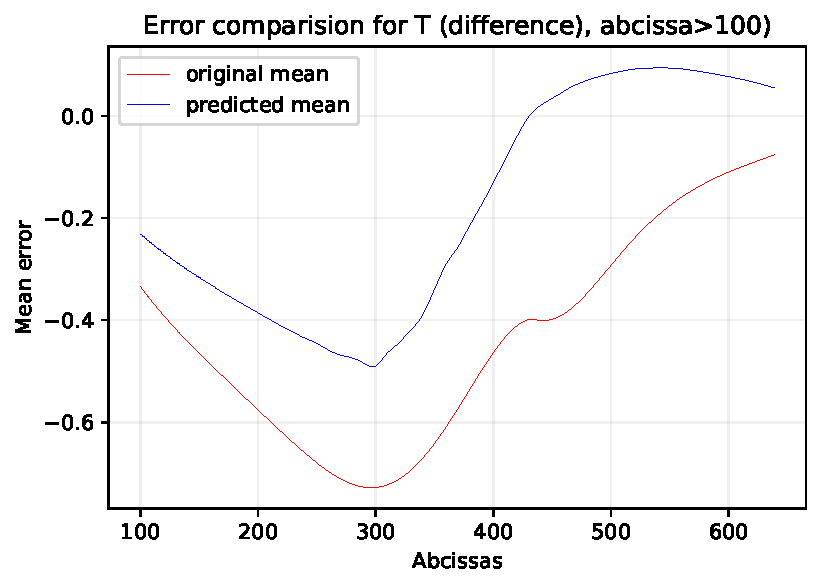
\includegraphics[width=\textwidth]{figures/T_error_comparison_after100_filipa.pdf}
        \caption{Baseline model}
        \label{fig:t_error_filipa}
    \end{subfigure}
    \hfill
    \begin{subfigure}[]{0.48\textwidth}
        \centering
        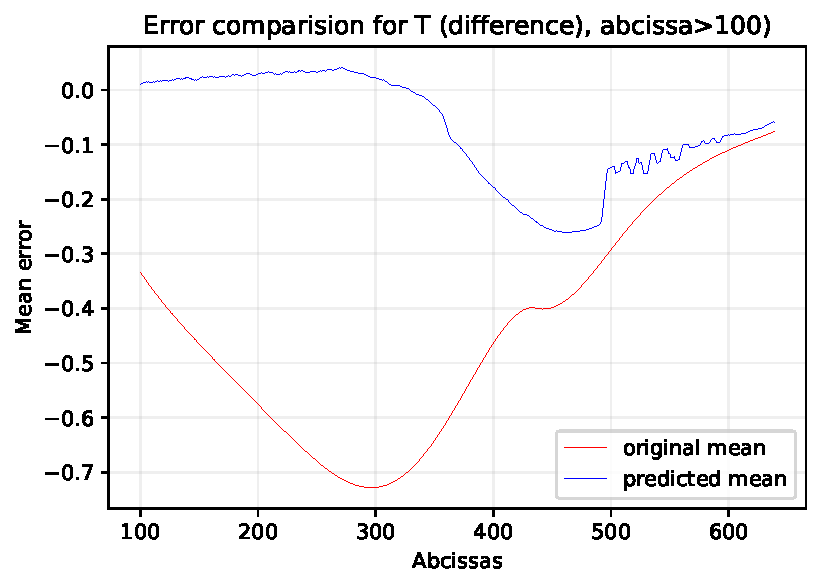
\includegraphics[width=\textwidth]{figures/T_error_comparison_after100_clusters.pdf}
        \caption{Clustering models}
        \label{fig:t_error_cluster}
    \end{subfigure}
\end{figure}

Figure \ref{fig:t_error_filipa} compares the baseline predictions for the $T [MK]$ variable with the original expert estimates. The baseline shows a slight decrease in the mean error in line with the original guesses. The clustering models (Figure \ref{fig:t_error_cluster}) faired much better than the baseline model, with initial estimates for the temperature being much closer to the simulation results.

%The clustering models faired better in the first 300 abscissas when compared to the baseline, with a significantly smaller mean error measured in this range. Unexpectedly, the mean error for the following abscissas increases substantially (in absolute value), even surpassing the ones measured on the original estimates. This might indicate that the models learned the initial features of the $T [MK]$ lines very well but failed to capture the complexities of the features measured from 300> like the other models.

Despite having provided initial flow estimates closer to the final simulation solution, the new estimates failed to reduce the overall computation time of MULTI-VP. The baseline model had a mean speedup of 1.06 over the initial method of running MULTI-VP with the expert initial flow guesses, while the new clustering approach yielded a speedup of 1.05.


\section{Summary}\label{sec:clustering_summary}
This chapter explained the use of clustering methods on solar wind profiles for improving initial flow estimates that were later tested on MULTI-VP. Sections \ref{sec:clustering_methods} and \ref{sec:validity_measures} provide an overview of the clustering methods and validity measures that were used. The multiple clustering approaches tested for this data are detailed in Section \ref{sec:clustering_experiments}. The choice of a single approach for testing is explained in \ref{sec:clustering_ml_experiments}, followed by the training process of the prediction models.

Lastly, Section \ref{sec:clustering_mulivp_results}, shows the results of the MULTI-VP simulation when the predictions from the new method are used as initial flow estimates. From there, it can be concluded that clustering the dataset and then training a separate model for each cluster generated estimates closer to the final solution of MULTI-VP. Unexpectedly, even with initial estimates closer to the final ones, the new approach failed to obtain a higher mean speedup than the baseline. 